\documentclass[a4paper,11pt]{article}
\usepackage[utf8]{inputenc}
\usepackage{hyperref}
\usepackage[french]{babel}
\usepackage{graphicx}
\usepackage{float}

%opening
\title{Barathon: rapport intermédiaire}
\author{Bourguignon Maxime \\ Jacobi Jordan \\ Simon Christophe \\ Vanneste Jean}

\begin{document}

\maketitle


\section*{Introduction}

Dans ce document, nous allons aborder plusieurs aspects de notre projet appelé \og{} Barathon\fg{}. Ce rapport intermédiaire est composé de plusieurs parties qui sont:

\begin{itemize}
 \item Description du projet;
 \item Diagrammes réalisés;
 \item Conventions de codage;
 \item Critères de qualité.
\end{itemize}

Ce document n'est pas exhaustif mais est assez représentatif de l'idée que nous nous faisons de notre application.

\section{Description du projet}

Le projet \og{} Barathon \fg{} doit permettre à un utilisateur de trouver facilement des bars à proximité et de se constituer un itinéraire. L'application est pensée pour tenir compte des préférences de l'utilisateur telles que les évévements, le budget, sa position géographique, ... Elle est pensée pour être déployée en tant qu'application mobile.

Après la création d'un profil de préférences, l'utilisateur pourra se servir de notre algorithme pour trouver le parcours qui correspond le mieux à ses critères.

Pour l'aspect base de données, nous souhaitons utiliser une DB noSQL de type graphe (neo4j) qui s'intègre particulièrement bien avec notre projet et le langage de programmation imposé qu'est le java.\\
L'idée est de parcourir le graphe en comparant les critères de l'utilisateur et les caractéristiques des lieux pour retourner les plus adéquats.

Pour l'implémentation, nous allons utiliser le design pattern Srategy qui se prête bien aux deux types de recherches qui sont:
\newline

\begin{itemize}
 \item Trouver un lieu à proximité;
 \item Trouver un itinéraire parcourant différents établissements.
\end{itemize}

\section{Diagrammes réalisés}

Dans cette section, vous trouvez ci-dessous les deux diagrammes réalisés sur le projet.

\subsection{Diagramme des cas d'utilisation}

\begin{figure}[H]
    \centering
    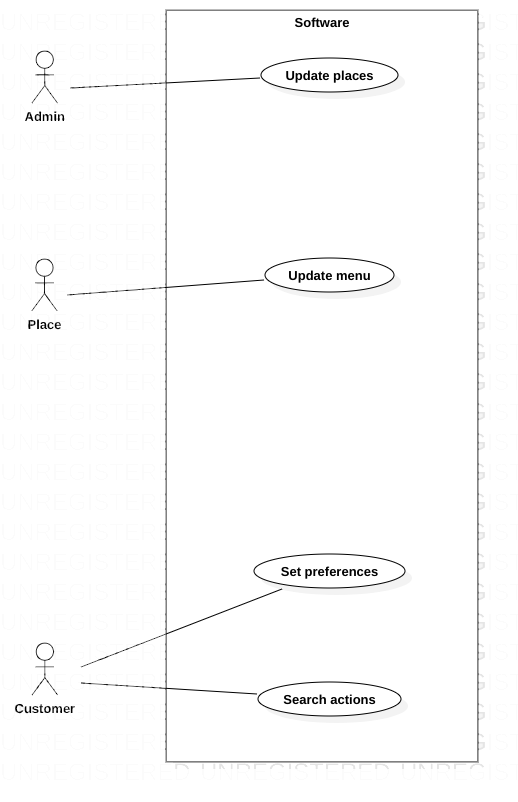
\includegraphics{UseCaseDiagram1.png}
    \caption{Diagramme des cas d'utilisation du projet Barathon}
\end{figure}


\subsection{Diagramme de classes}

\begin{figure}[H]
    \centering
    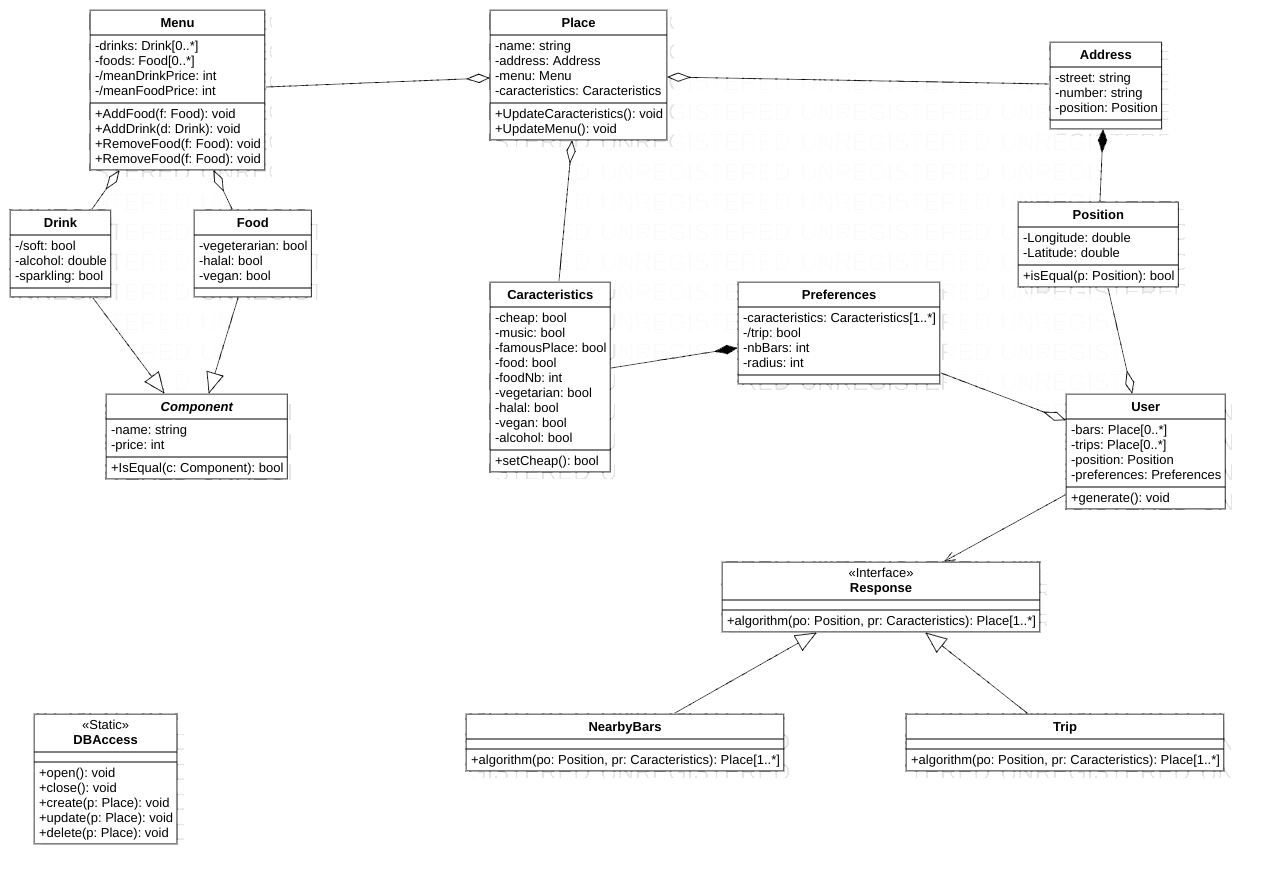
\includegraphics[width=\textwidth]{ClassDiagram.png}
    \caption{Diagramme de classes du projet Barathon}
\end{figure}

\section{Conventions de codage}

Pour les conventions de codage, nous allons utiliser les conventions de codage standard de java.
Cela nous permettra de vérifier facilement que notre code respecte celles-ci avec des applications tels que PMD ou Checkstyle.\\
Les conventions de codage standard de java que nous suivont sont celles-ci:

\begin{itemize}
  \item Le nom des classes est en camelcase avec la première lettre en majuscule;
  \item Le nom des variables est en camelcase avec la première lettre en minuscule;
  \item Les variables d'une seule lettre sont utilisées localement;
  \item Le nom des constantes est en majuscule avec un underscore pour séparer les mots;
  \item Le nom des fichiers en minuscule avec des tirets pour séparer les noms;
  \item L'indentation est de 4 espaces;
  \item Les commentaires se trouvent au dessus des déclarations de classes.
\end{itemize}

\newpage
Pour de plus amples informations, vous pouvez retrouver nos conventions de codage sur le site d'oracle:
\url{https://www.oracle.com/technetwork/java/codeconvtoc-136057.html}.

\section{Critères de qualité}

Comme critères de qualité, nous avons choisi:
\begin{itemize}
  \item Une densité de commentaires située entre vingt et trente pour cent;
  \item Une couverture de code de quarante pour cent au minimum pour la partie \og{} logique \fg{};
  \item Une rapidité d'exécution : exécution de l'algorithme de recherche d'itinéraire en moins de 30 secondes sur un téléphone mobile Android de dernière génération.
\end{itemize}


Il s'agit d'un travail que nous devrons échanger. Pour faciliter la relève, nous voulons un programme qui est bien documenté, et qui est composé de fonctions fiables.\\
Pour notre projet, une application de recherche dans une database, nous voulons que celle-ci s'exécute vite.
Cette vitesse va dépendre de la requête et du hardware, mais nous voulons optimiser celle-ci le plus possible.

\section*{Conclusion}
Nous nous rendons déjà compte que choisir des critères de qualité n'est pas chose aisée.\\
Nous espérons proposer un projet intéressant pour nos futurs successeurs.

\end{document}
